\documentclass{beamer}

\usepackage[utf8]{inputenc}
\usepackage{pdfpages}
\usepackage{listings}


%Information to be included in the title page:
\title{Foreman Provisioning}
\author{Emerson Ford}
\date{}



\begin{document}
\frame{\titlepage}

\begin{frame}
	\frametitle{What is Foreman?}

\end{frame}

\begin{frame}
	\frametitle{Use Cases for Foreman}

\end{frame}

\begin{frame}[fragile]
	\frametitle{Custom iPXE Image}
	\flushleft
	Near vanilla iPXE image with the following embedded script:

	\centering
	\begin{lstlisting}[language=bash,frame=single,basicstyle=\fontsize{4}{6pt}\selectfont]
#!ipxe
# Intermediate iPXE script to report MAC address to Foreman

:net0
isset ${net0/mac} || goto no_nic
dhcp net0 || goto net1
chain http://fm-test.chpc.utah.edu/unattended/iPXE?mac=${net0/mac} || goto net1

:net1
isset ${net1/mac} || goto no_nic
dhcp net1 || goto net2
chain http://fm-test.chpc.utah.edu/unattended/iPXE?mac=${net1/mac} || goto net2

...


:net33
goto no_nic

exit 0

:no_nic
echo Failed to chainload from any network interface
sleep 30
exit 1
  \end{lstlisting}

\end{frame}

\begin{frame}[fragile]
	\frametitle{Foreman iPXE Workflow}

	\begin{columns}
		\begin{column}{0.5\textwidth}
			\flushleft
			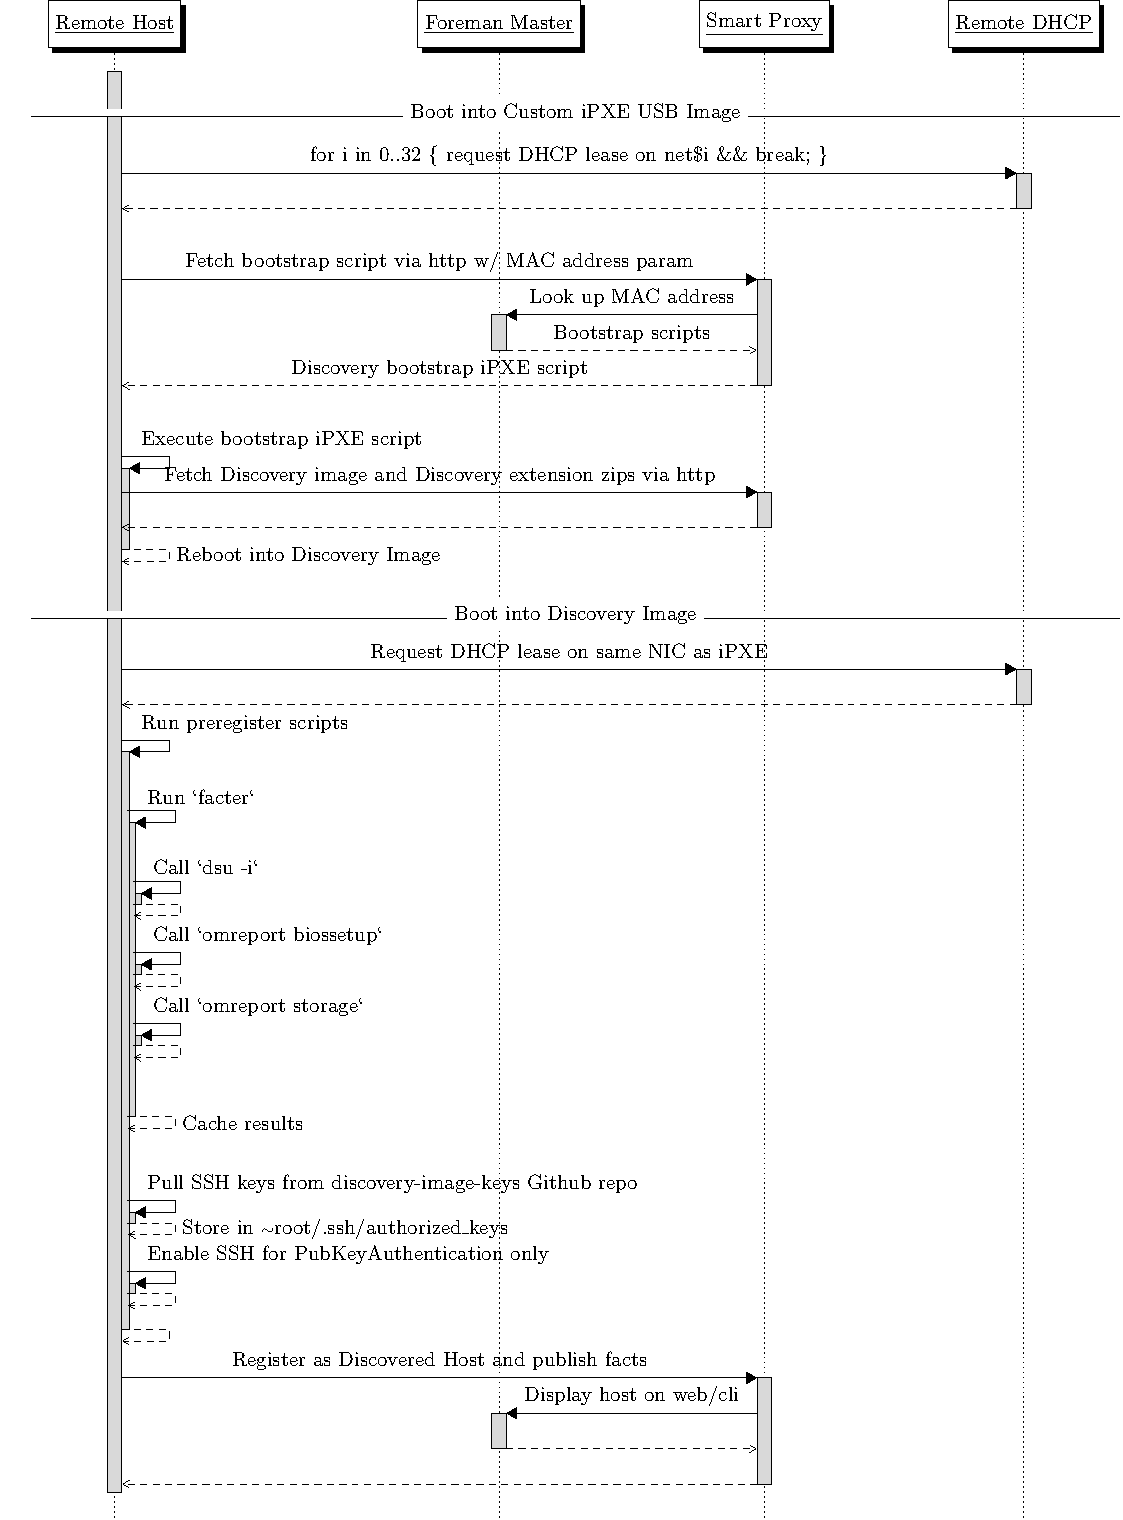
\includegraphics[width=\textwidth,height=\textheight-15mm,keepaspectratio]{discovery_sd}
		\end{column}

		\begin{column}{0.5\textwidth}
			Boot into Custom iPXE Image can happen in two ways:
			\begin{itemize}
				\item USB boot with custom iPXE image.
				\item PXE boot into custom iPXE image (configure DHCP):
				      \begin{lstlisting}[frame=single,basicstyle=\fontsize{3.5}{6pt}\selectfont]
if exists user-class and option user-class = "iPXE" {
  filename "http://fm-test.chpc.utah.edu/unattended/iPXE?bootstrap=1";
} elsif option architecture = 00:06 {
  filename "ipxe.efi";
} elsif option architecture = 00:07 {
  filename "ipxe.efi";
} elsif option architecture = 00:09 {
  filename "ipxe.efi";
} else {
  filename "undionly.0";
}
          \end{lstlisting}
			\end{itemize}
		\end{column}
	\end{columns}
\end{frame}

\begin{frame}[fragile]
	\frametitle{Foreman Installation Workflow}

	\centering
	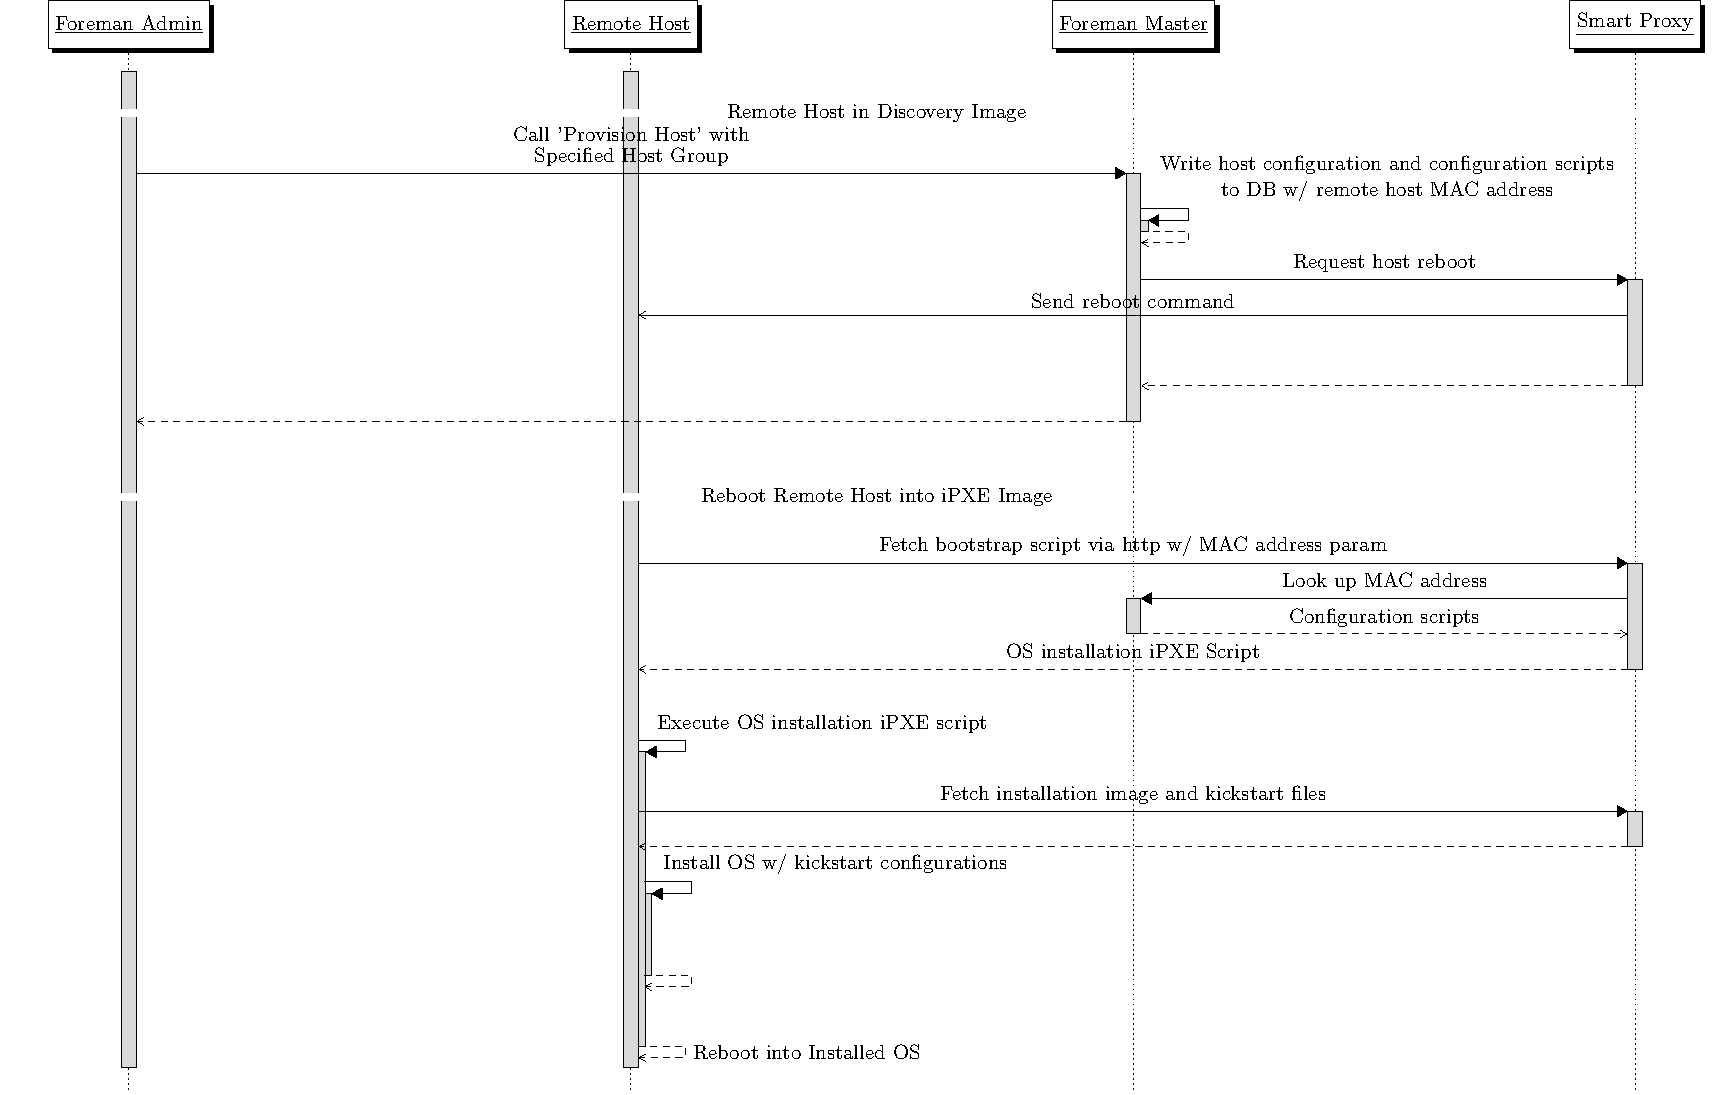
\includegraphics[width=\textwidth,height=\textheight-15mm,keepaspectratio]{installation_sd}
	\tiny
	Foreman supports kickstart files (RedHat), preseed files (Debian), etc.

\end{frame}

\begin{frame}[fragile]
	\frametitle{Foreman Configuration Workflow}

	\centering
	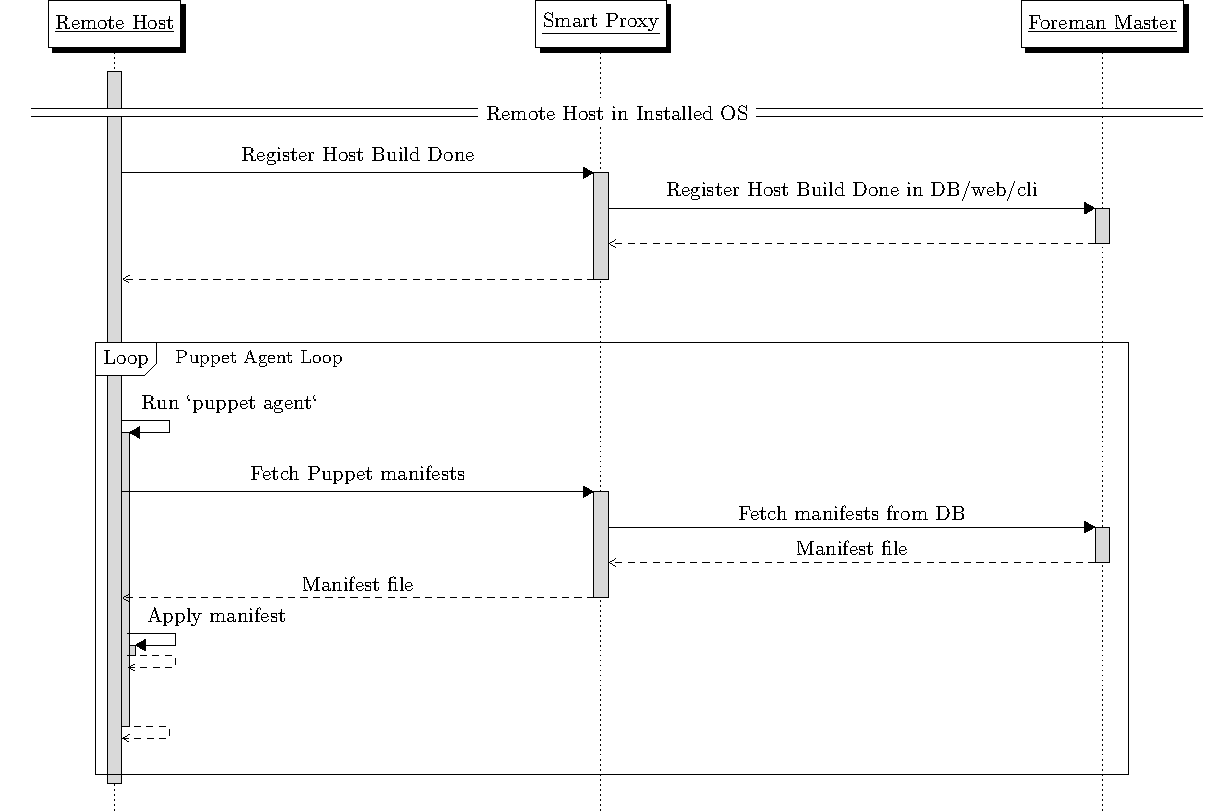
\includegraphics[width=\textwidth,height=\textheight-15mm,keepaspectratio]{configuration_sd}
	\tiny
	Foreman comes with Puppet by default but can be configured with Ansible, SaltStack, etc.

\end{frame}



\end{document}
